\documentclass[11pt,english]{article}
\usepackage{babel}
\usepackage{verbatim}
\usepackage{float}
\usepackage{amsmath}
\usepackage{amssymb}
\usepackage[left=2.7cm,right=2.7cm,top=2.7cm,bottom=2.7cm]{geometry}
\usepackage{graphicx}
\usepackage{subcaption}

\setlength{\parindent}{0pt}
\newcommand{\reffig}[1]{Figure \ref{#1}\hspace{2pt}}


\begin{document}
Kun Zhou \hfil UID: 204688165	
	
P1. \\
i) I think step 3 is more efficient than step 2, because with $\sigma_0=1$, the $p(x,y)$ is very small when $\pi(x,y)$ is large.  So It is hard for step 2 to get sample with more useful information.

\begin{figure}[H]
	\includegraphics[height=5in, width=0.8\textwidth]{p1_1.pdf}
	\caption{$\hat{\theta}$ against n} \label{p1_1}
\end{figure}

From \reffig{p1_1}, we can see $\hat{\theta}_1$ of step 1 quickly converges to 4 after sampling amount increase to $10^5$.  For step 2, $\hat{\theta}_2$ are prone to converge to 4, but the estiamted values are not stable even when $N=10^{15}$.  For step 3, $\hat{\theta}_3$ converges to 4 after the amount increases to $10^{10}$.  So step 1 is the best method and step 3 is better than step 2.\\
ii)\\
First calculate the $ess(n)$ for step 2 and step 3.\\
\begin{flalign*}
&\omega = \frac{\pi(x, y)}{p(x,y)}&\\
&E[\omega] = E[\frac{\pi(x, y)}{p(x,y)}] = \int \frac{\pi(x, y)}{p(x,y)}p(x,y) dxdy = 1&\\
&E[\omega^2] = E[\frac{\pi(x, y)^2}{p(x,y)^2}] = \int \frac{\pi(x, y)^2}{p(x,y)}dxdy = \int \frac{\sigma_0^2}{2\pi}e^{-\left[ (x-2)^2+(y-2)^2-\frac{1}{2\sigma_0^2}(x^2+y^2)\right]} dxdy&\\
&= \int \frac{\sigma_0^2}{2\pi} e^{-\left[ (1-\frac{1}{2\sigma_0^2})x^2 - 4x + (1-\frac{1}{2\sigma_0^2})y^2 - 4y + 8 \right]} dxdy&\\
&= \int \frac{\sigma_0^2}{2\pi} e^{-(1-\frac{1}{2\sigma_0^2})\left[x - \frac{4\sigma_0^2}{2\sigma_0^2-1} \right]^2 + \frac{8\sigma_0^2}{2\sigma_0^2-1}}e^{-(1-\frac{1}{2\sigma_0^2})\left[y - \frac{4\sigma_0^2}{2\sigma_0^2-1} \right]^2 + \frac{8\sigma_0^2}{2\sigma_0^2-1}}e^{-8}dxdy&\\
&=\frac{\sigma_0^2}{2\pi}(\sqrt{\frac{\pi}{\frac{2\sigma_0^2-1}{2\sigma_0^2}}})^2e^{\frac{16\sigma_0^2}{2\sigma_0^2-1}}e^{-8}&\\
&=\frac{\sigma_0^4}{2\sigma_0^2-1}e^{\frac{8}{2\sigma_0^2-1}}&\\
&\Rightarrow ess(n) = \frac{n}{1+Var[\omega]} = \frac{n}{E[\omega^2]} = \frac{2\sigma_0^2-1}{\sigma_0^4}e^{\frac{-8}{2\sigma_0^2-1}}n&
\end{flalign*}
For step 2, $\sigma_0=1 \Rightarrow ess(n) = e^{-8}n=0.000335n$.  For step 3, $\sigma_0=4 \Rightarrow ess(n)=0.09355n.$\\
For $ess^{*}$, calculating one $\hat{\theta}$ is not enough to estimate errors, so calculate $\hat{\theta}$ at least 500 times for each step and then calculate the standard deviation of each estimate.  If 2 steps have a similar standard deviation, the estimated errors could be regarded as same.  For example, if $n_1=5$, the standard deviation of step 1 is 0.6282757.  For step 2, $n_2=210000$, the standard deviation of step 2 is 0.5757558.  So we can think $ess^*(n_1) = ess^*(n_2)$ and theoretical value $n_2 = 5 * e^8 = 14904$.
\begin{figure}[H]
	\centering
	\begin{subfigure}[b]{0.475\textwidth}
		\centering
		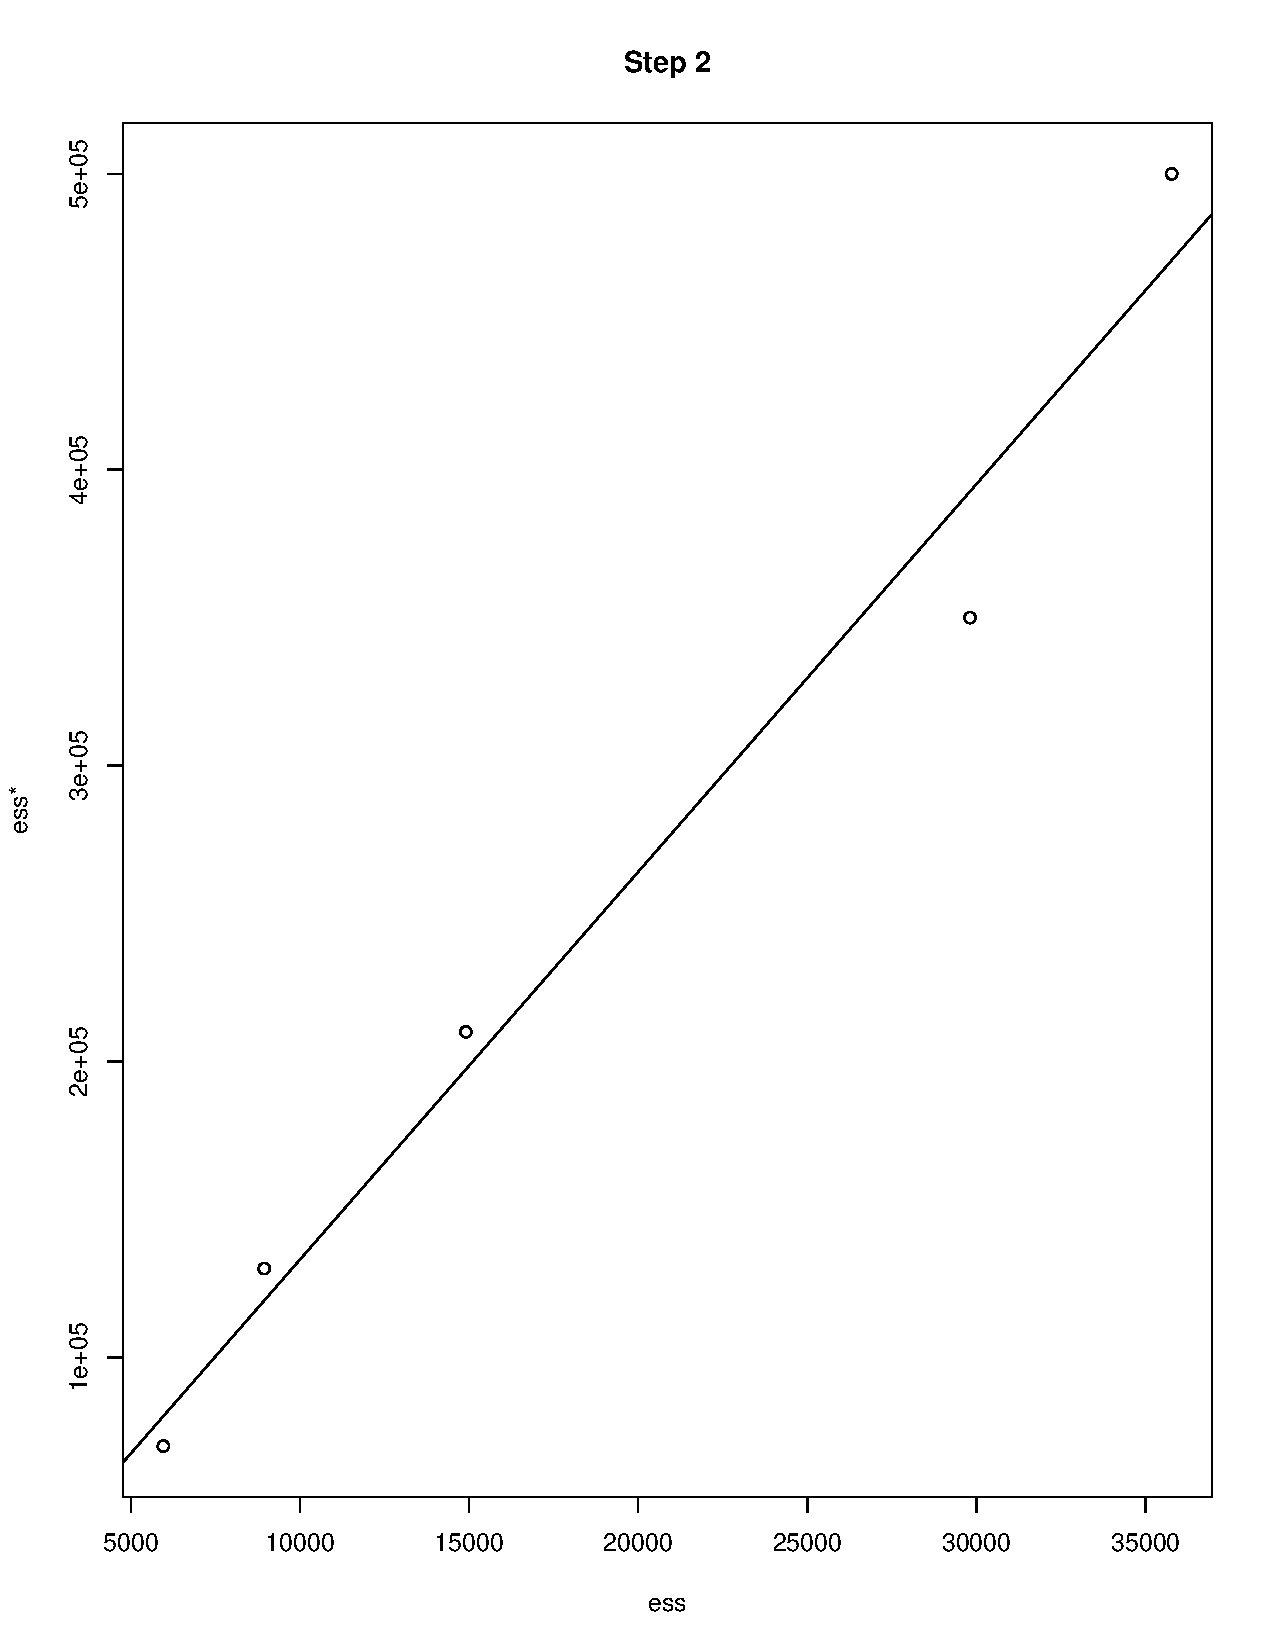
\includegraphics[width=\textwidth, height=6cm]{p1_2.pdf}
		\caption{step 2}\label{p1_2}
	\end{subfigure}
	\quad
	\begin{subfigure}[b]{0.475\textwidth}
		\centering
		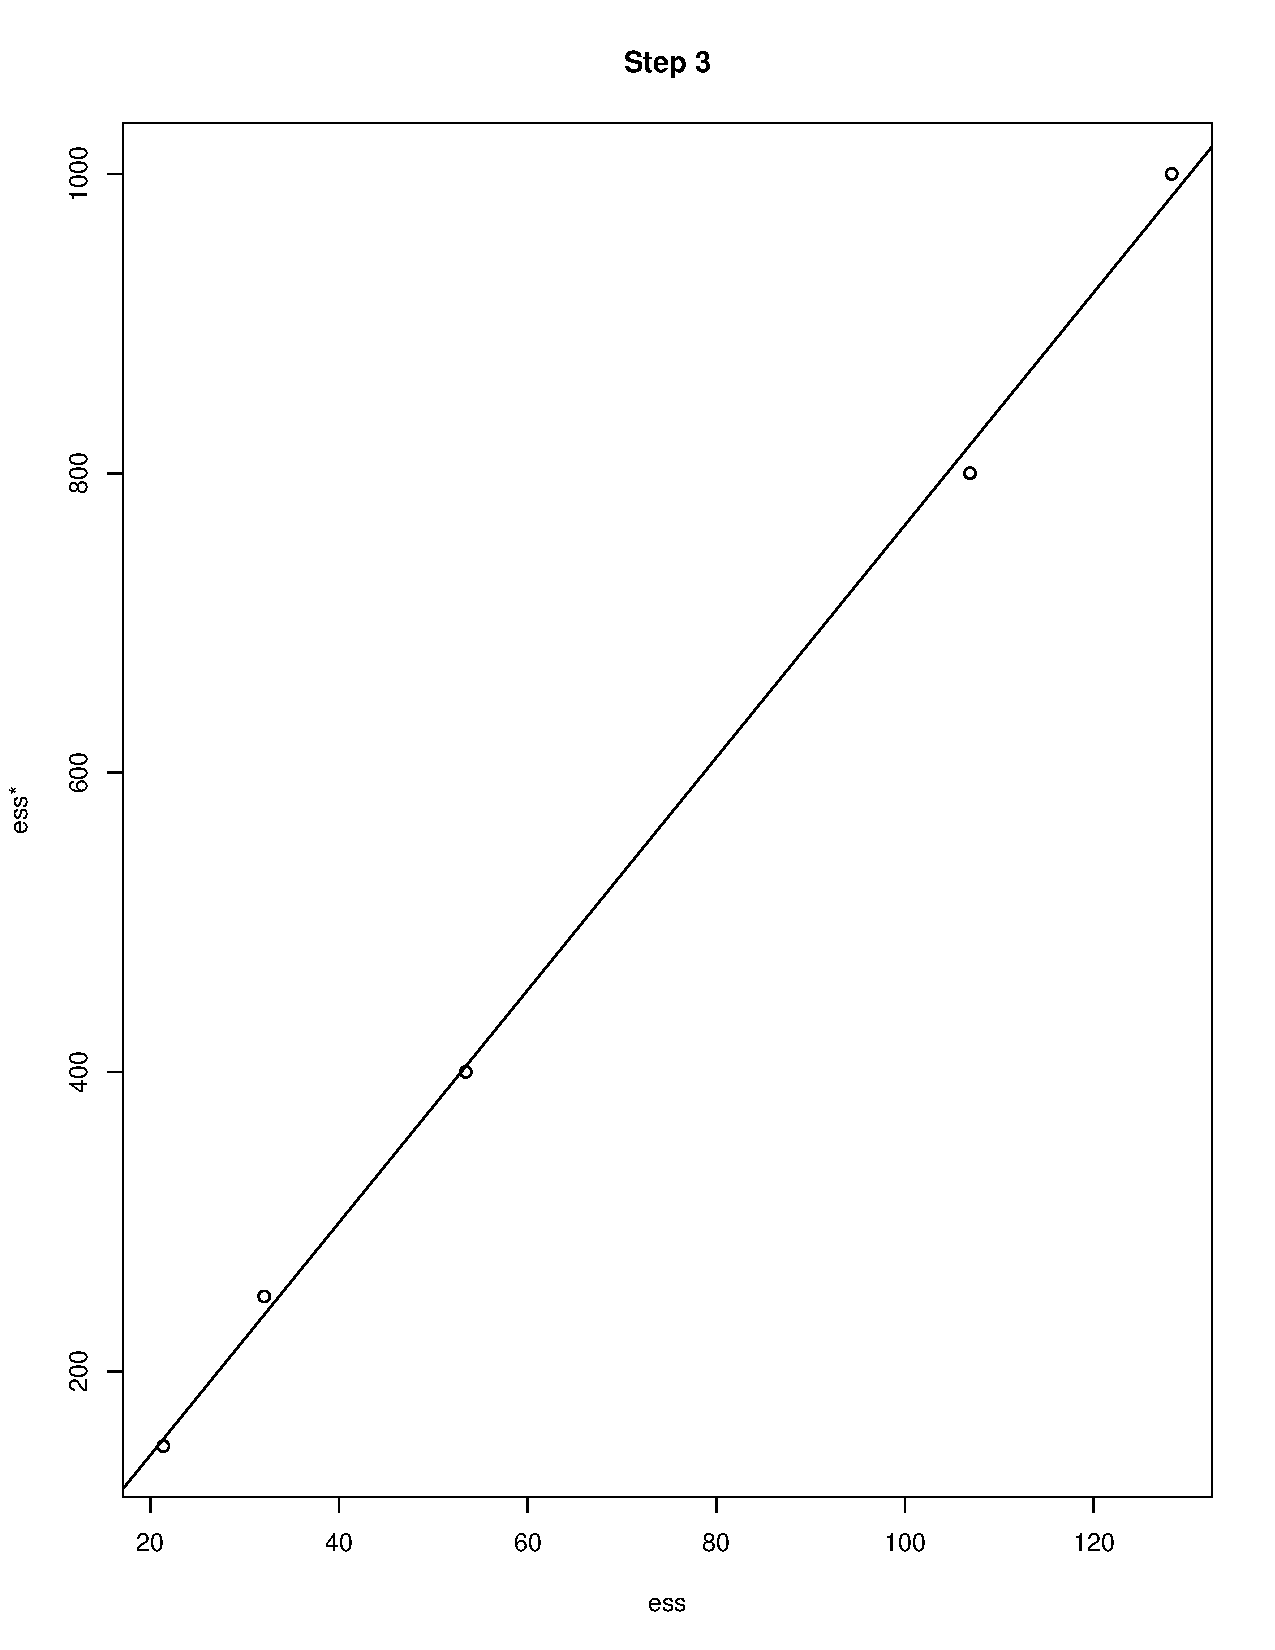
\includegraphics[width=\textwidth, height=6cm]{p1_3.pdf}
		\caption{step 3}\label{p1_3}
	\end{subfigure}
	\caption{}
\end{figure}
We can see $ess$ and $ess^*$ are proportional for both step 2 and step 3.  From \reffig{p1_2} and \reffig{p1_3}, if we want step 2 and step 3 have the same effecive sample size, step 2 requires much more samples.\\
The following is R code.\\
\begin{verbatim}
library(MASS)
library(Rcpp)
sourceCpp("C:\\Study\\Statistics\\202C Monte Carlo Methods for
Optimization\\project1\\project1.cpp")

theta.est <- function(mu, sigma, n, tar_mu, tar_sigma)
{
sample = mvrnorm(n, mu=mu, Sigma=sigma)
ones = matrix(1, nrow=nrow(sample))
tar_temp = (sample - ones %*% t(tar_mu)) %*% solve(tar_sigma)
tar_den = exp(applet(tar_temp, (t(sample) - tar_mu %*% t(ones))) / -2) /
sqrt(det(tar_sigma))
apr_temp = (sample - ones %*% t(mu)) %*% solve(sigma)
apr_den = exp(applet(apr_temp, (t(sample) - mu %*% t(ones))) / -2) /
sqrt(det(sigma))
result = tar_den / apr_den * sample %*% matrix(c(1,1))
return(mean(result))
}

tar_mu = matrix(c(2,2))
tar_sigma = diag(2)

#step1
mu1 = matrix(c(2,2))
sigma1 = diag(2)
n1=c()
result1=c()
for(i in seq(from=1, to=16, by=0.5))
{
n1 = c(n1, floor(exp(i)))
result1 = c(result1, theta.est(mu, sigma, floor(exp(i)), tar_mu, tar_sigma))
}
plot(log(n1), result1)

#step2
mu2 = matrix(c(0, 0))
sigma2 = diag(c(1, 1))
n2=c()
result2=c()
for(i in seq(from=1, to=16, by=0.5))
{
n2 = c(n2, floor(exp(i)))
result2 = c(result2, theta.est(mu2, sigma2, floor(exp(i)), tar_mu, tar_sigma))
}
plot(log(n2), result2)

#step3
mu3 = matrix(c(0, 0))
sigma3 = diag(c(1, 1))*16
n3=c()
result3=c()
for(i in seq(from=1, to=16, by=0.5))
{
n3 = c(n3, floor(exp(i)))
result3 = c(result3, theta.est(mu, sigma, floor(exp(i)), tar_mu, tar_sigma))
}
plot(log(n3), result1, type="l", col=1, lty=1, xlim=c(0, 17), ylim=c(0, 14),
xlab="log(N)", ylab="estimated theta")
points(log(n2), result2, type="l", col=2, lty=2)
points(log(n3), result3, type="l", col=4, lty=4)
legend(14, 14, legend=c("step 1", "step 2", "step 3"), col=c(1,2,4), lty=c(1,2,4))
\end{verbatim}\\
\vspace{2em}
The following are the C++ codes.
\begin{verbatim}
NumericMatrix applet(NumericMatrix x, NumericMatrix y)
{
NumericMatrix result = NumericMatrix(x.nrow(), 1);
for(int i=0; i<x.nrow(); i++)
{
result(i, 0) = 0;
for(int j=0; j<x.ncol(); j++)
{
result(i, 0) = result(i, 0) + x(i, j) * y(j, i);
}
}
return result;
}
\end{verbatim}

P2.\\
Method 1: I use probability $g_1(x)=\displaystyle\prod_{j=1}^m\frac{1}{k_j}$, where $m$ is the total length of the path, and $k_j$ is the number of possible choices at j-th step.\\
Method 2: I introduce an early termination rate $\epsilon=0.05$ at each step (while in textbook, $\epsilon=0.1$). So $g_2(x) = \displaystyle\prod_{j=1}^m\frac{1}{k_j*0.95}$.\\
Method 3: For any walk that longer than 50, $u=5$ more children based on it are generated and are reweighed by $\omega_0 = \frac{\omega}{u}.$\\
i)\\
\begin{figure}[H]
	\centering
	\begin{subfigure}[b]{0.475\textwidth}
		\centering
		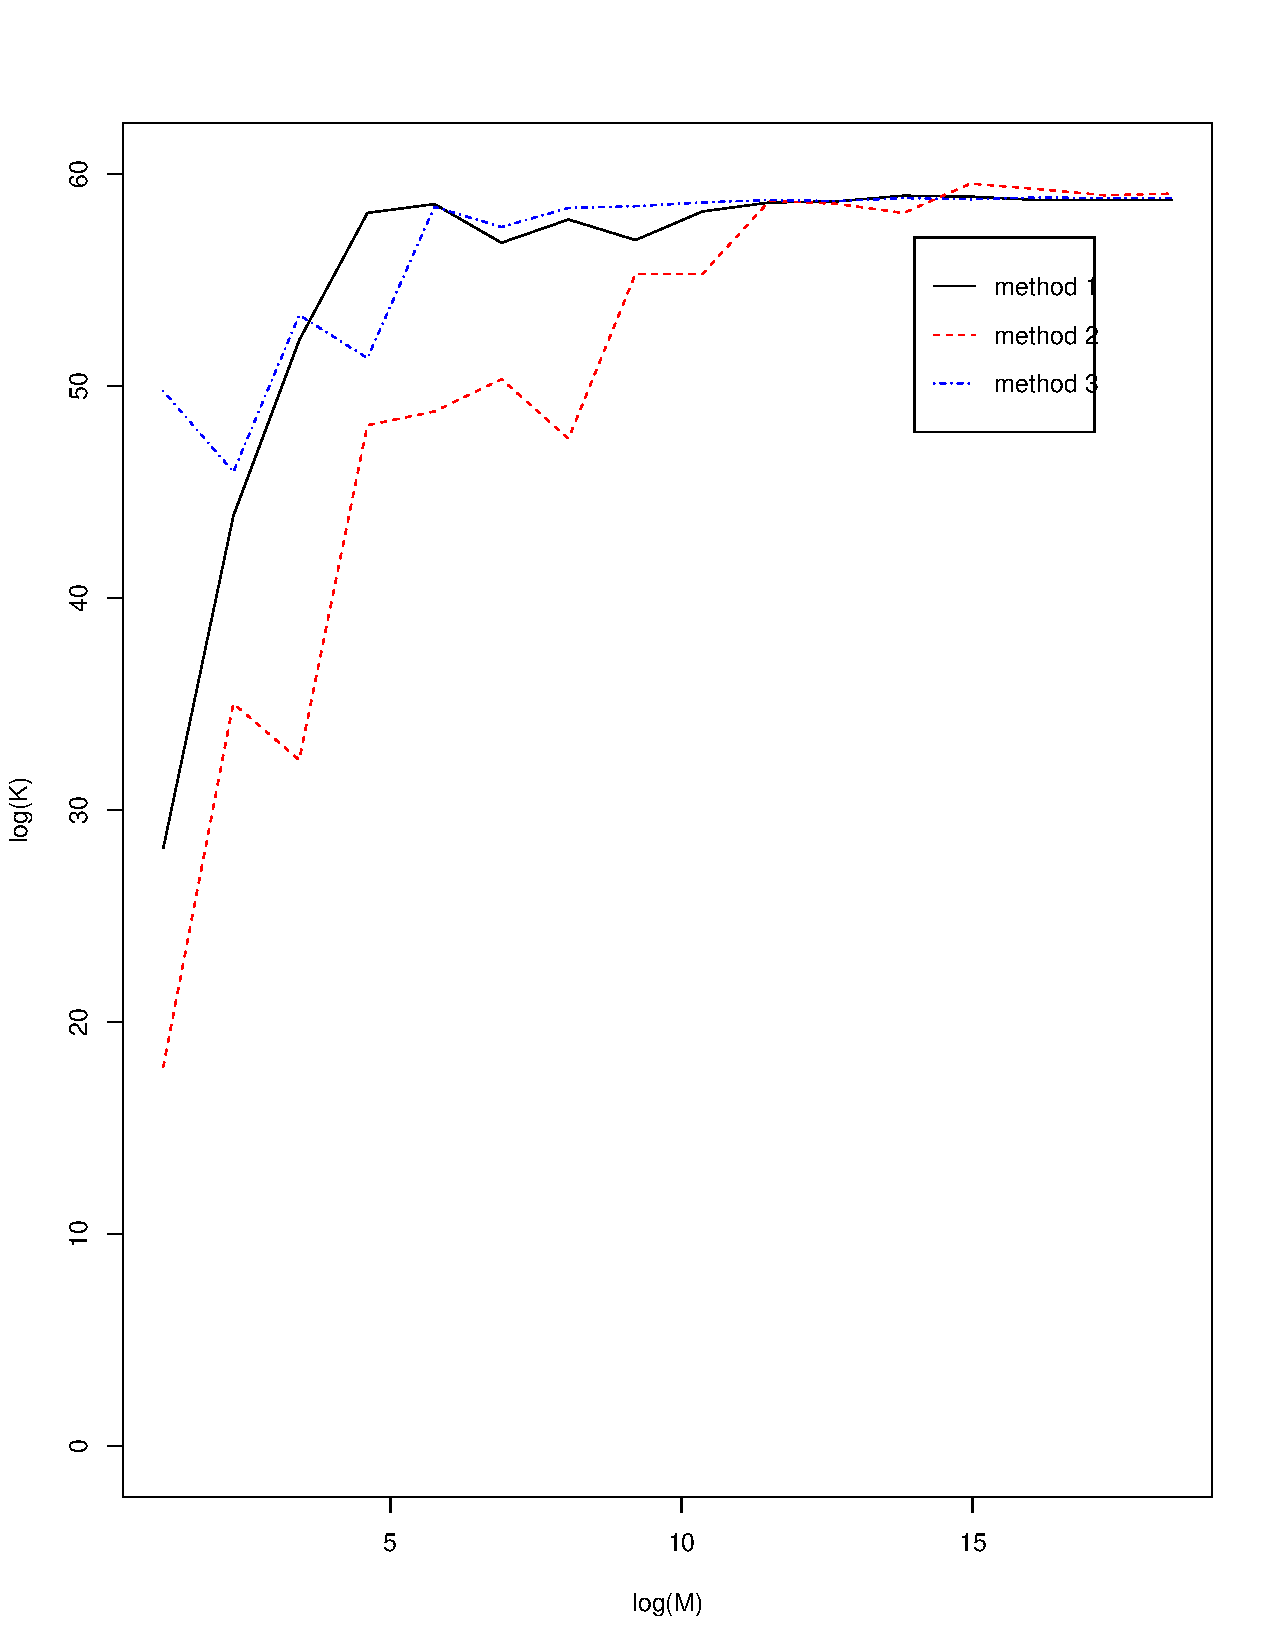
\includegraphics[width=\textwidth, height=6cm]{p2_1_1.pdf}
		\caption{Global log-log plot of K against M}\label{p2_1_1}
	\end{subfigure}
	\quad
	\begin{subfigure}[b]{0.475\textwidth}
		\centering
		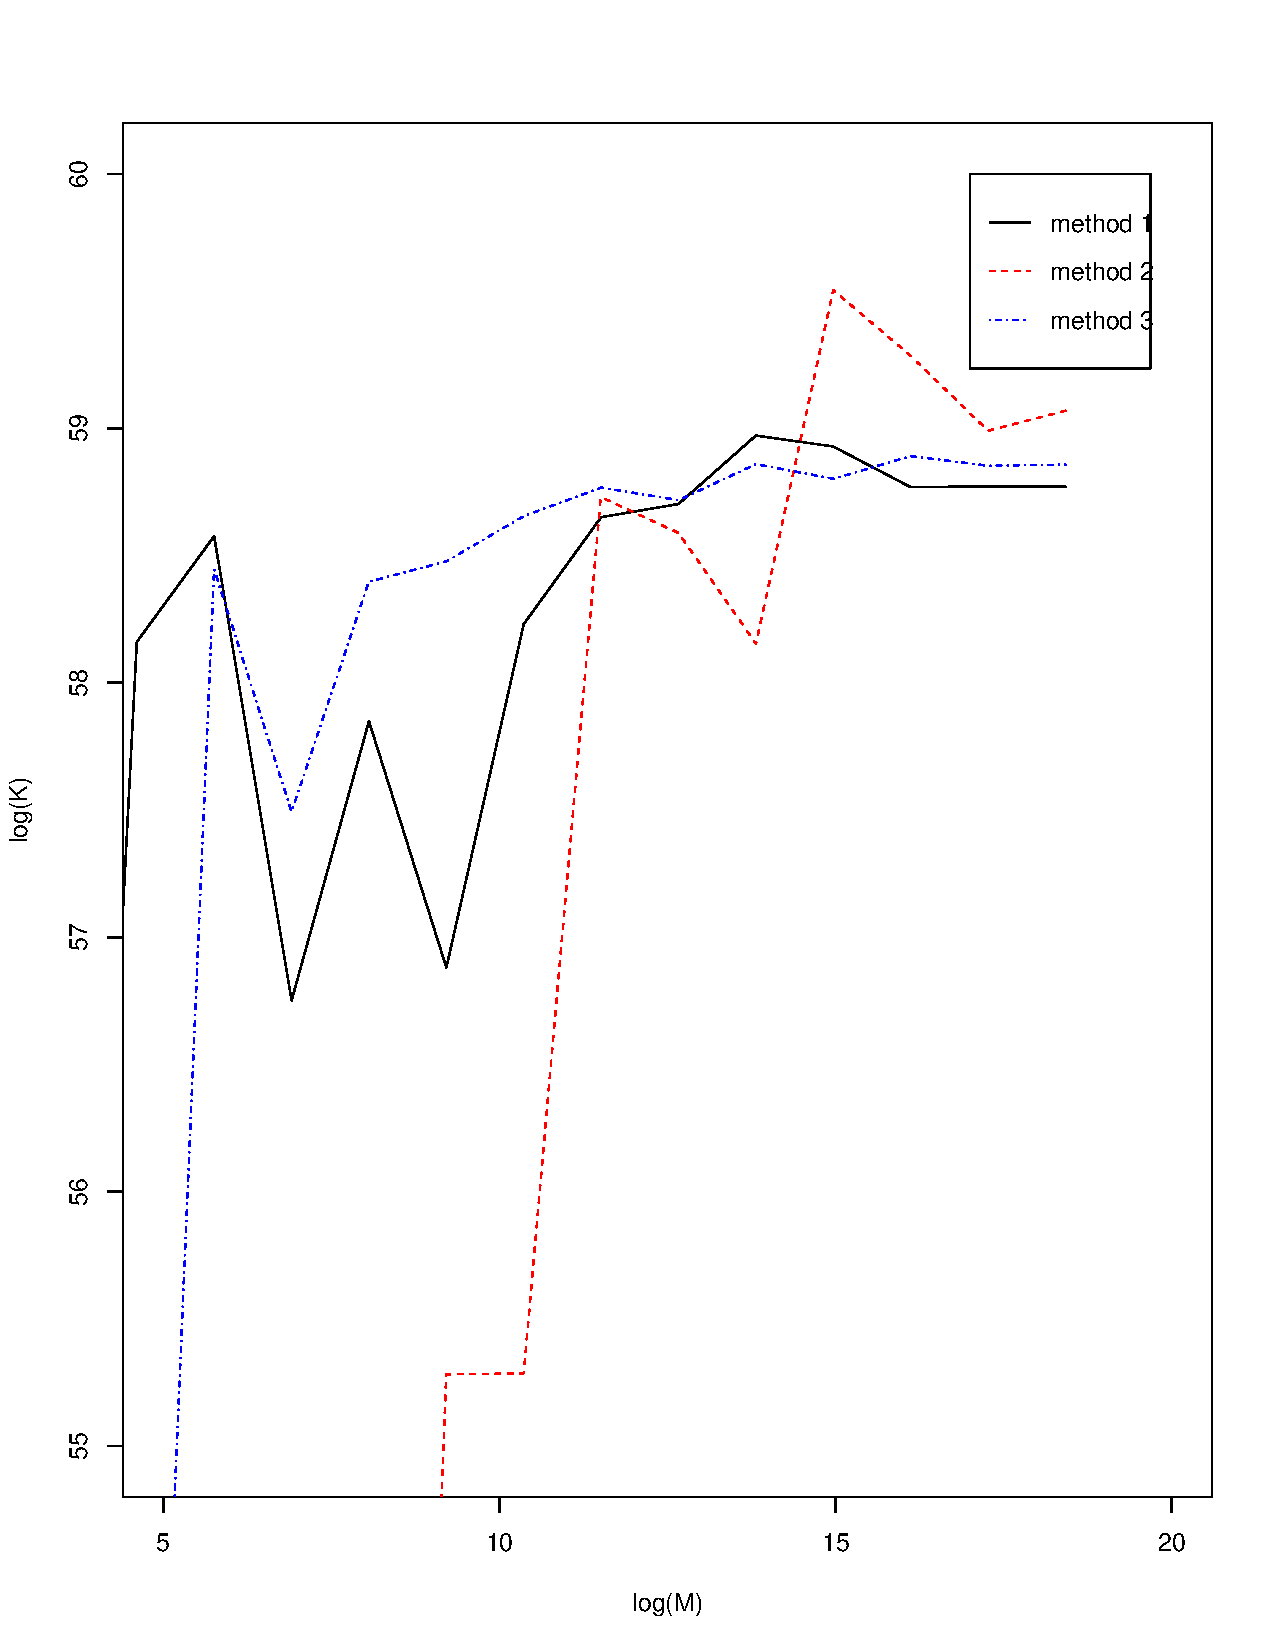
\includegraphics[width=\textwidth, height=6cm]{p2_1_2.pdf}
		\caption{Local log-log plot of K against M}\label{p2_1_2}
	\end{subfigure}
	\caption{}
\end{figure}

From \reffig{p2_1_1}, we can see that SIS processes of all 3 methods are converging with M increasing. \reffig{p2_1_2} demonstrates that Method 3 converges the fastest and Method 2 converges the most slowly. The limit values of Method 2 and Method 3 are higher than Method 1, which means the bias cannot be neglected. The following are the estimated value of $K$s when $M=10^8$ for the 3 methods respectively: $3.316744 * 10^{25}, \quad  4.512596*10^{25}, \quad 3.649155*10^{25}$.\\



ii)\\
I applied the method mentioned in textbook.\\
$1.501552*10^{24}$

iii)
\begin{figure}[H]
	\centering
	\begin{subfigure}[b]{0.475\textwidth}
		\centering
		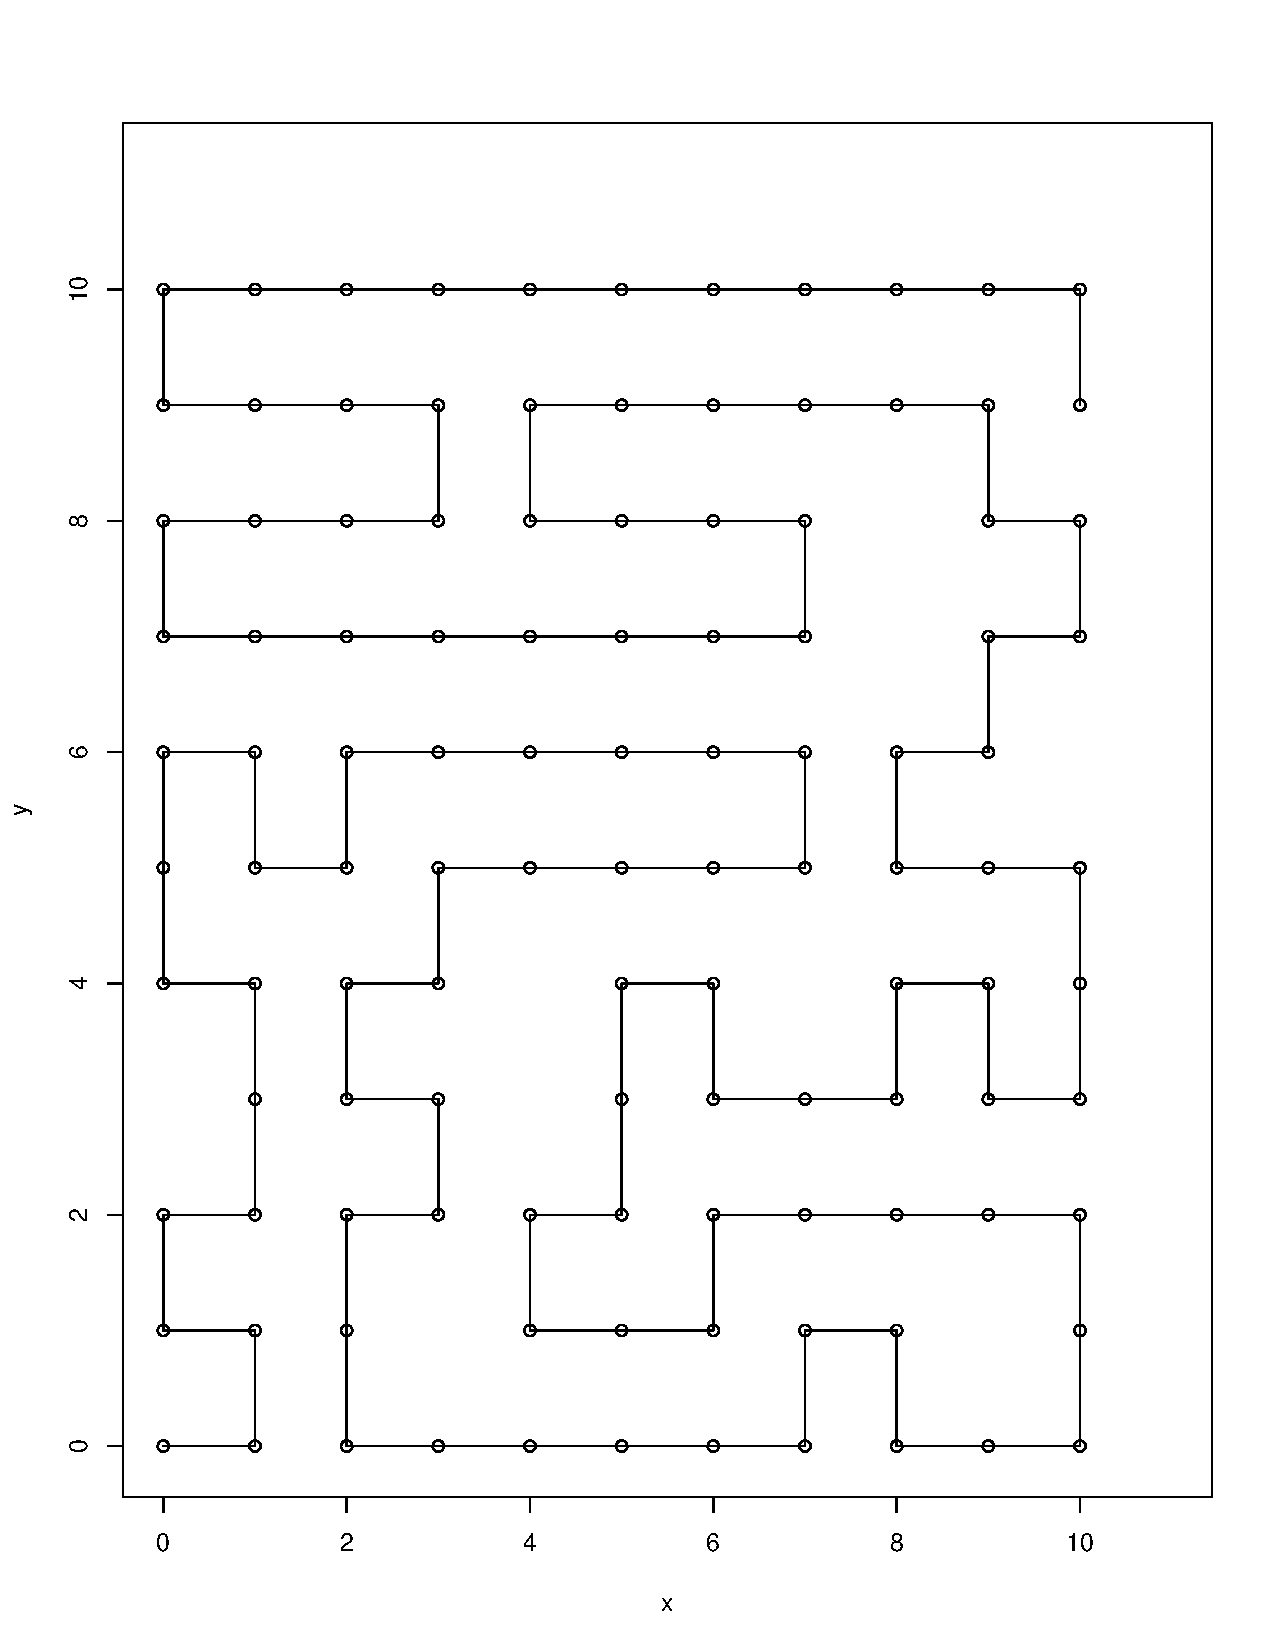
\includegraphics[width=\textwidth, height=6cm]{p2_3_1_111.pdf}
		\caption{Longest path}\label{p2_3_1_111}
	\end{subfigure}
	\quad
	\begin{subfigure}[b]{0.475\textwidth}
		\centering
		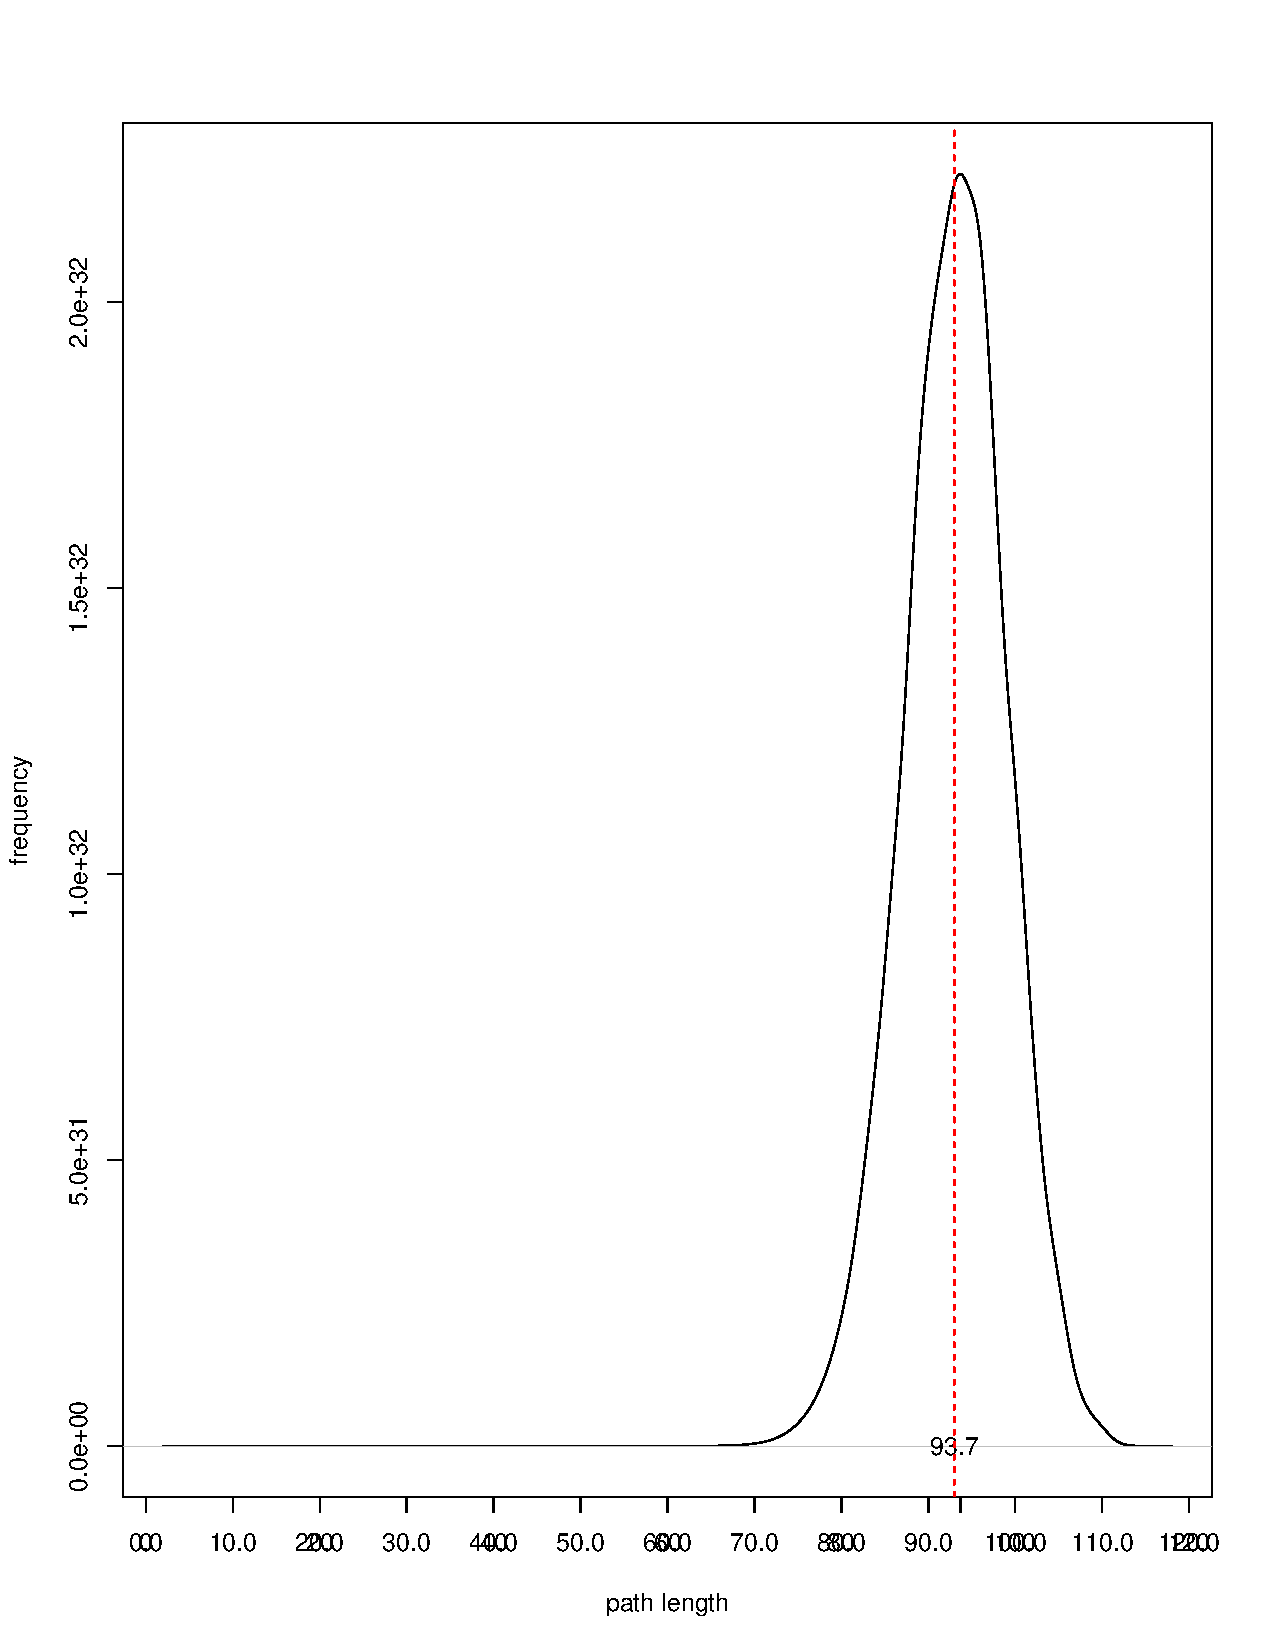
\includegraphics[width=\textwidth, height=6cm]{p2_3_2.pdf}
		\caption{Density function of paths}\label{p2_3_2}
	\end{subfigure}
	\caption{Method 1}
\end{figure}
For Method 1, \reffig{p2_3_1_111} has length 111.  \\
\begin{figure}[H]
	\centering
	\begin{subfigure}[b]{0.475\textwidth}
		\centering
		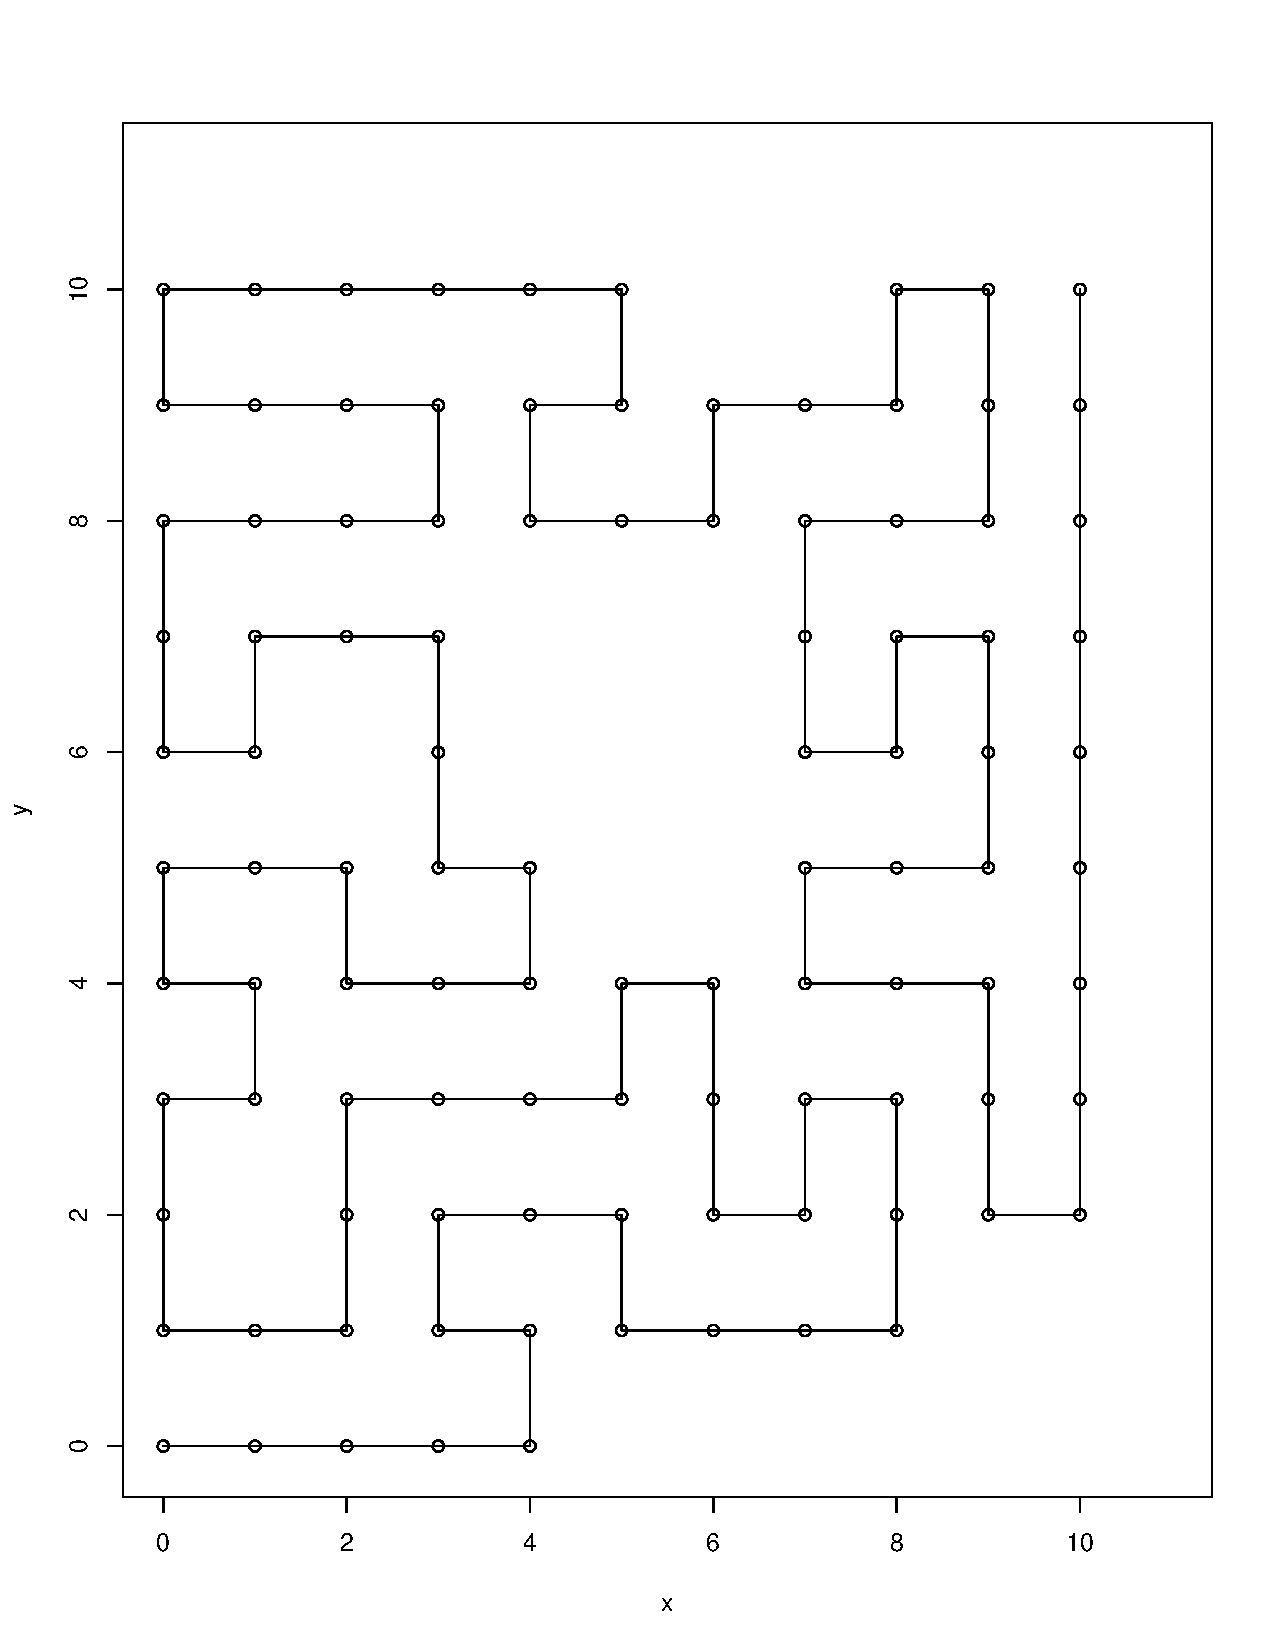
\includegraphics[width=\textwidth, height=6cm]{p2_3_3_100.pdf}
		\caption{Longest path}\label{p2_3_3_100}
	\end{subfigure}
	\quad
	\begin{subfigure}[b]{0.475\textwidth}
		\centering
		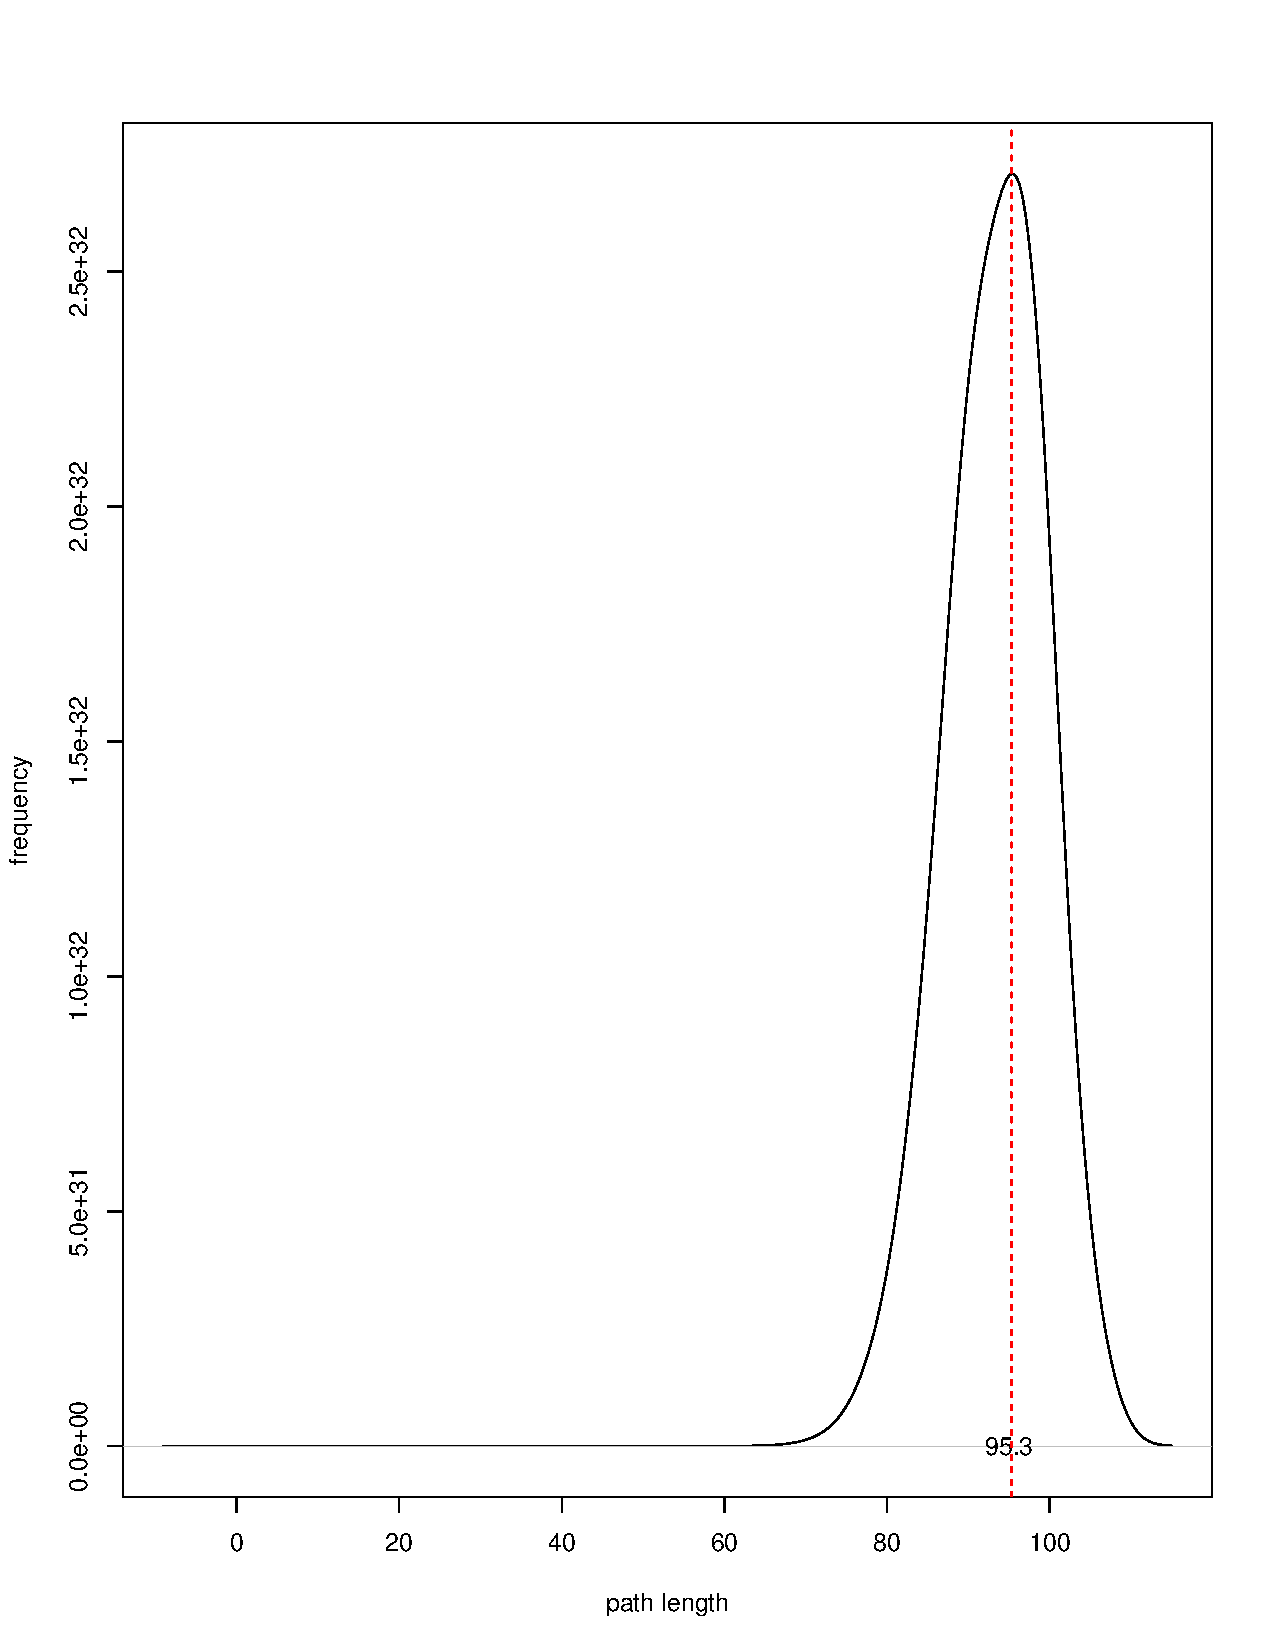
\includegraphics[width=\textwidth, height=6cm]{p2_3_4.pdf}
		\caption{Density function of paths}\label{p2_3_4}
	\end{subfigure}
	\caption{Method 2}
\end{figure}
For Method 2, \reffig{p2_3_3_100} has length 100. \reffig{p2_3_4} is against intuition.  The most dense point is 95.3 while the length of the longest path for Method 2 is 100. But it's reasonable, because $\frac{1}{\epsilon}^m$ makes longer paths' weight much more larger. \\

\begin{figure}[H]
	\centering
	\begin{subfigure}[b]{0.475\textwidth}
		\centering
		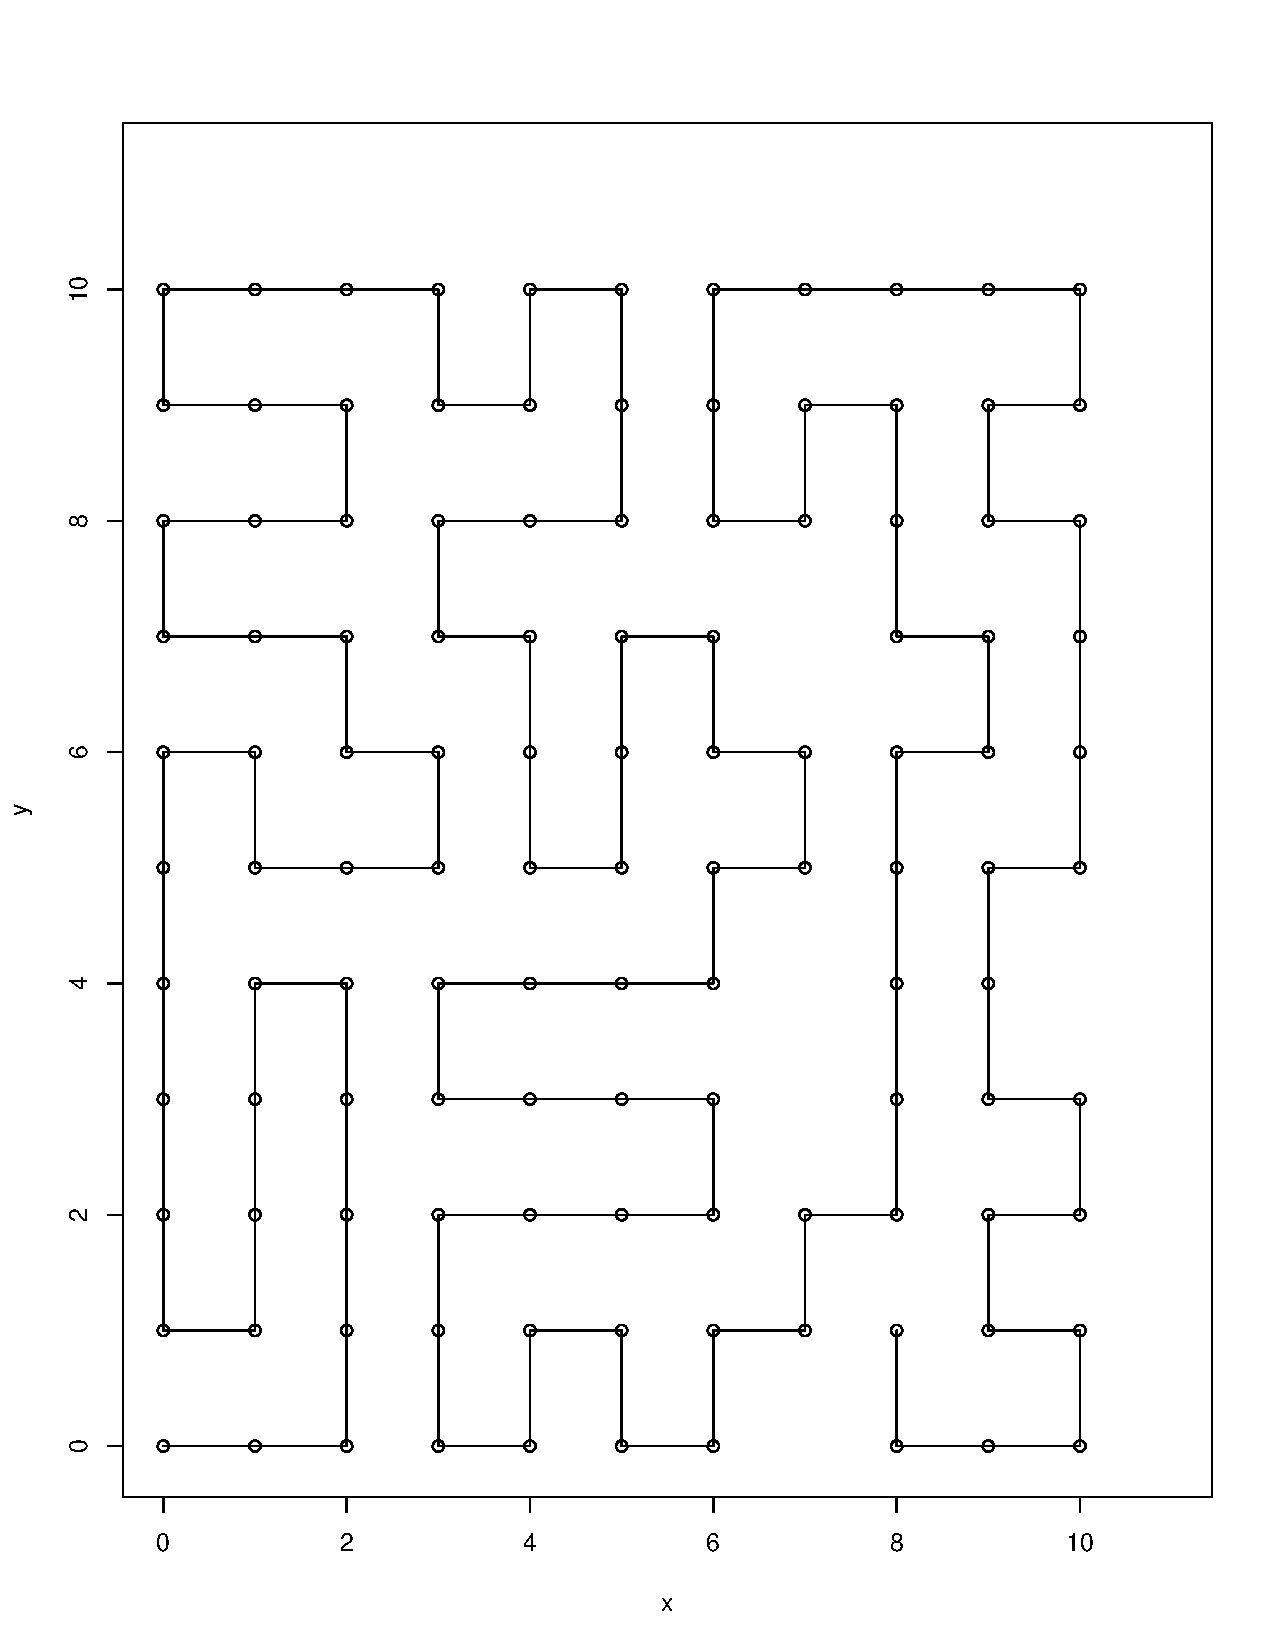
\includegraphics[width=\textwidth, height=6cm]{p2_3_5_115.pdf}
		\caption{Longest path}\label{p2_3_5_115}
	\end{subfigure}
	\quad
	\begin{subfigure}[b]{0.475\textwidth}
		\centering
		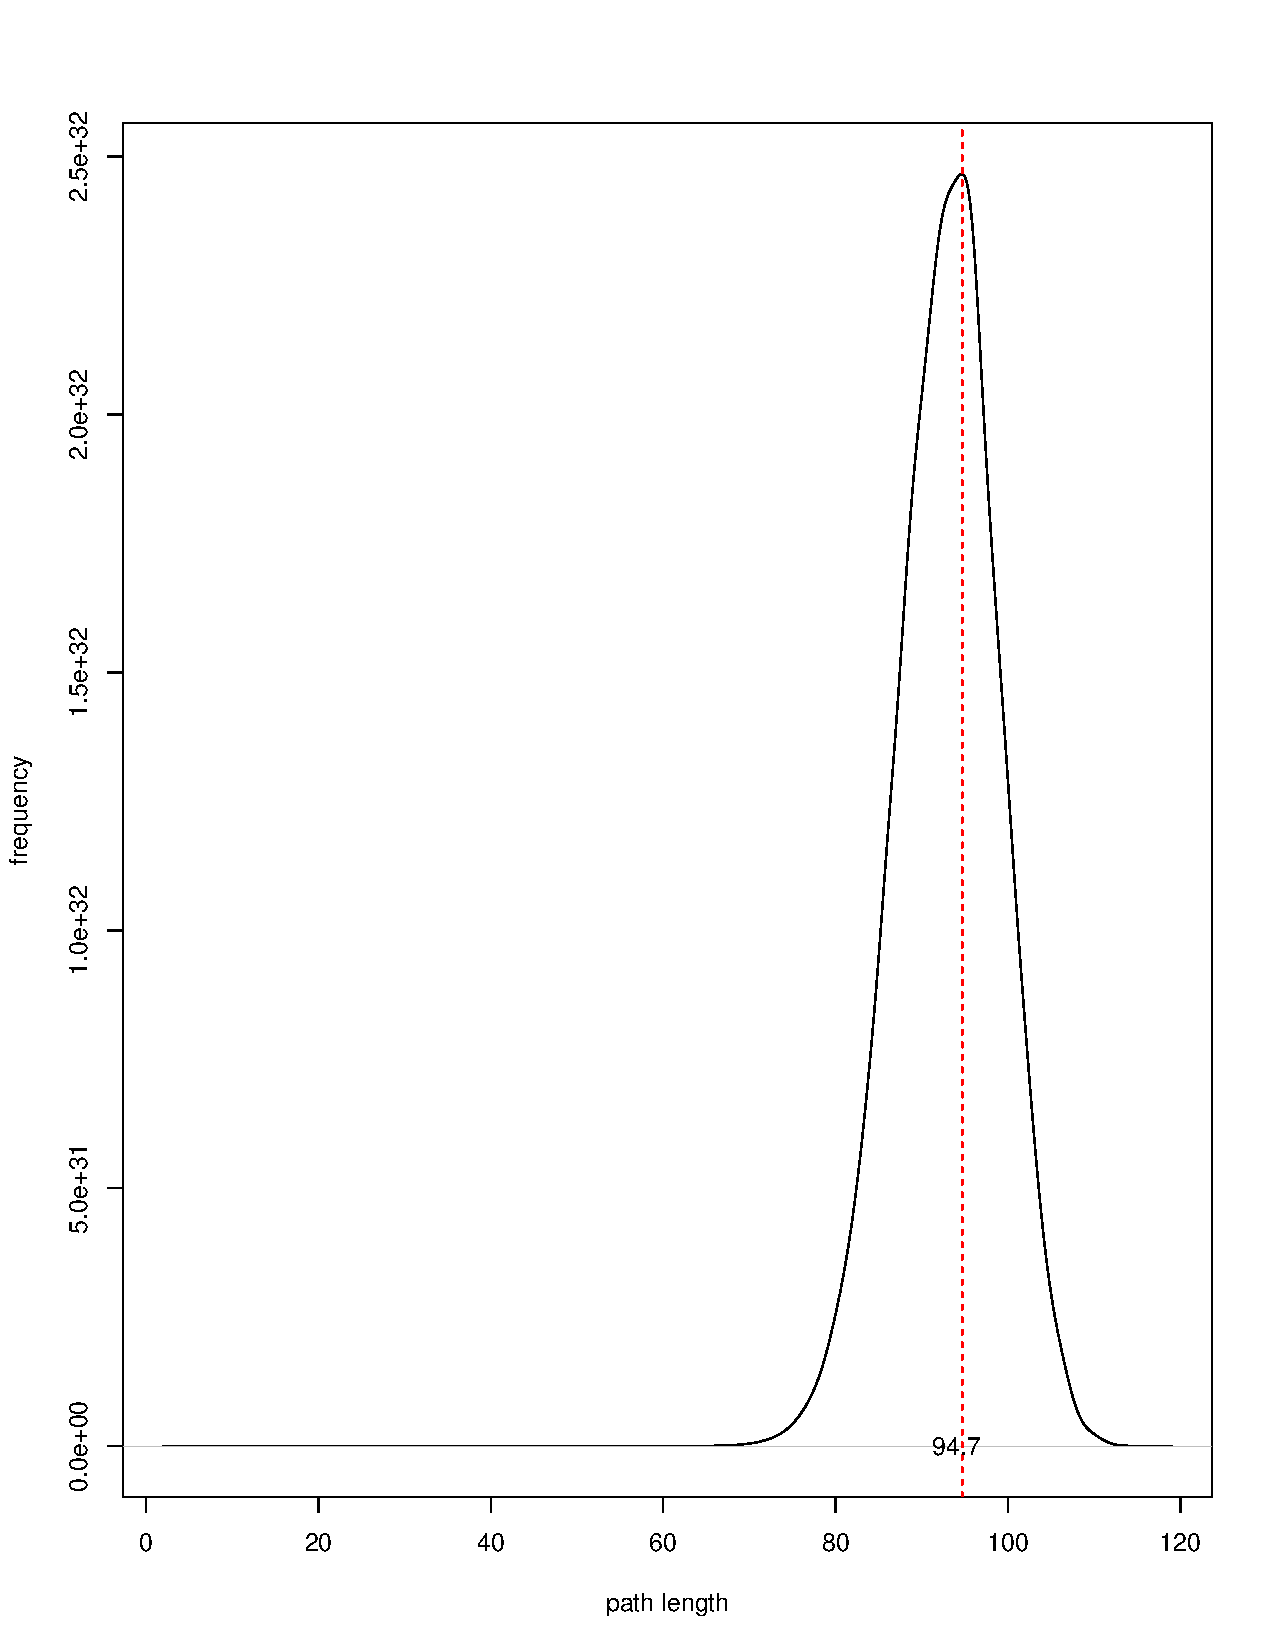
\includegraphics[width=\textwidth, height=6cm]{p2_3_6.pdf}
		\caption{Density function of paths}\label{p2_3_6}
	\end{subfigure}
	\caption{Method 3}
\end{figure}

For Method 3, \reffig{p2_3_5_115} has length 115. The most dense point is 94.7 which is a little higher than the one of Method 1, becuase there are more paths, having length more than 50 and some of which are adapted to new weights.
	
The following are C++ codes for all questions.
\begin{verbatim}
#include <Rcpp.h>
#include<cstdlib>
#include <time.h> 
#include <math.h>
using namespace Rcpp;

NumericMatrix applet(NumericMatrix x, NumericMatrix y)
{
NumericMatrix result = NumericMatrix(x.nrow(), 1);
for(int i=0; i<x.nrow(); i++)
{
result(i, 0) = 0;
for(int j=0; j<x.ncol(); j++)
{
result(i, 0) = result(i, 0) + x(i, j) * y(j, i);
}
}
return result;
}


class SinglePath
{
public:
SinglePath();
SinglePath(double _epsilon);
SinglePath(int _x, int _y, bool _stop, int _Length, double _probInv, int
 _arrive[][13], int _cor_x[], int _cor_y[]);
void Simulate();

int printX();
int printY();
double printProbInv();
int printL();
bool printStop();
void printCor_x(int _cor_x[]);
void printCor_y(int _cor_y[]);
void printArrive(int _arrive[][13]);
void OneStep();
NumericMatrix printCor();

private:
int x;
int y;
bool stop;
int Length;
int arrive[13][13];
double probInv;
double epsilon;

int cor_x[200];
int cor_y[200];

};

SinglePath::SinglePath()
{
x = 1;
y = 1;
stop = false;
Length = 0;
probInv = 1;
for (int i = 0; i<13; i++)
{
for (int j = 0; j<13; j++)
{
if (i == 0 || j == 0 || i == 12 || j == 12)
arrive[i][j] = 1;
else
arrive[i][j] = 0;
}
}
epsilon = 0;
for (int i = 1; i<200; i++)
cor_x[i] = 0;
for (int i = 1; i<200; i++)
cor_y[i] = 0;
cor_x[0] = 1;
cor_y[0] = 1;

}
SinglePath::SinglePath(double _epsilon)
{
x = 1;
y = 1;
stop = false;
Length = 0;
probInv = 1;
for (int i = 0; i<13; i++)
{
for (int j = 0; j<13; j++)
{
if (i == 0 || j == 0 || i == 12 || j == 12)
arrive[i][j] = 1;
else
arrive[i][j] = 0;
}
}
epsilon = _epsilon;
for (int i = 1; i<200; i++)
cor_x[i] = 0;
for (int i = 1; i<200; i++)
cor_y[i] = 0;
cor_x[0] = 1;
cor_y[0] = 1;
}
SinglePath::SinglePath(int _x, int _y, bool _stop, int _Length, double
 _probInv, int _arrive[][13], int _cor_x[], int _cor_y[])
{
x = _x;
y = _y;
stop = _stop;
Length = _Length;
probInv = _probInv;
for (int i = 0; i<13; i++)
{
for (int j = 0; j<13; j++)
{
if (i == 0 || j == 0 || i == 12 || j == 12)
arrive[i][j] = 1;
else
arrive[i][j] = _arrive[i][j];
}
}
epsilon = 0;
for (int i = 0; i<200; i++)
cor_x[i] = _cor_x[i];
for (int i = 0; i<200; i++)
cor_y[i] = _cor_y[i];
}
void SinglePath::OneStep()
{
if (stop)
return;
bool direction[] = { arrive[x][y + 1] == 0, arrive[x][y - 1] == 0, arrive[x
 - 1][y] == 0, arrive[x + 1][y] == 0 };//up down left right
int count = direction[0] + direction[1] + direction[2] + direction[3];
if (count == 0)
{
stop = true;
return;
}
if (rand() * 1.0 / RAND_MAX < epsilon)
{
stop = true;
return;
}
Length++;
probInv = probInv * count / (1 - epsilon);
int direct = rand() % count;
int index = -1;
int value = -1;
while (value != direct)
{
index++;
value += direction[index];
}
arrive[x][y] = 1;
switch (index) {
case 0: y = y + 1; break;
case 1: y = y - 1; break;
case 2: x = x - 1; break;
case 3: x = x + 1; break;
}
cor_x[Length] = x;
cor_y[Length] = y;

}
void SinglePath::Simulate()
{
while (!stop)
OneStep();
}
int SinglePath::printX()
{
return x - 1;
}
int SinglePath::printY()
{
return y - 1;
}
double SinglePath::printProbInv()
{
return probInv;
}
int SinglePath::printL()
{
return Length;
}
bool SinglePath::printStop()
{
return stop;
}
void SinglePath::printCor_x(int _cor_x[])
{
for (int i = 0; i < 200; i++)
_cor_x[i] = cor_x[i];
}
void SinglePath::printCor_y(int _cor_y[])
{
for (int i = 0; i < 200; i++)
_cor_y[i] = cor_y[i];
}
void SinglePath::printArrive(int _arrive[][13])
{
for (int i = 0; i < 13; i++)
for (int j = 0; j < 13; j++)
_arrive[i][j] = arrive[i][j];
}
NumericMatrix SinglePath::printCor()
{
NumericMatrix result = NumericMatrix(2, 200);
for (int i = 0; i<200; i++)
{
if (i == 0 || cor_x[i] != 0 || cor_y[i] != 0)
{
result(0, i) = cor_x[i]-1;
result(1, i) = cor_y[i]-1;
}
else
{
result(0, i) = 0;
result(1, i) = 0;
}
}
return result;
}


class SinglePath50 : public SinglePath
{
public:
SinglePath50();
SinglePath50(double _epsilon);
void SimulateBefore50();

int printX_50();
int printY_50();
double printProbInv_50();
int printL_50();
bool printStop_50();
void printCor_x_50(int _cor_x[]);
void printCor_y_50(int _cor_y[]);
void printArrive_50(int _arrive[][13]);


private:
int x_50;
int y_50;
bool stop_50;
int Length_50;
int arrive_50[13][13];
double probInv_50;
int cor_x_50[200];
int cor_y_50[200];

};
SinglePath50::SinglePath50()
:SinglePath()
{}
SinglePath50::SinglePath50(double _epsilon)
: SinglePath(_epsilon)
{}
void SinglePath50::SimulateBefore50()
{
while (!printStop() && printL() < 50)
OneStep();
if (printL() == 50 && !printStop())
{
x_50 = printX();
y_50 = printY();
stop_50 = printStop();
Length_50 = printL();
printArrive(arrive_50);
probInv_50 = printProbInv();
printCor_x(cor_x_50);
printCor_y(cor_y_50);
}
}
int SinglePath50::printX_50()
{
return x_50;
}
int SinglePath50::printY_50()
{
return y_50;
}
double SinglePath50::printProbInv_50()
{
return probInv_50;
}
int SinglePath50::printL_50()
{
return Length_50;
}
bool SinglePath50::printStop_50()
{
return stop_50;
}
void SinglePath50::printCor_x_50(int _cor_x[])
{
for (int i = 0; i < 200; i++)
_cor_x[i] = cor_x_50[i];
}
void SinglePath50::printCor_y_50(int _cor_y[])
{
for (int i = 0; i < 200; i++)
_cor_y[i] = cor_y_50[i];
}
void SinglePath50::printArrive_50(int _arrive[][13])
{
for (int i = 0; i < 13; i++)
for (int j = 0; j < 13; j++)
_arrive[i][j] = arrive_50[i][j];
}






// [[Rcpp::export]]
NumericMatrix SAW1(long M)
{
NumericMatrix result = NumericMatrix(2, M);
SinglePath ex;
srand(time(NULL));
for(long i=0; i<M; i++)
{
ex = SinglePath();
ex.Simulate();
result(0, i) = ex.printProbInv();
result(1, i) = ex.printL();
}
return result;
}

// [[Rcpp::export]]
NumericMatrix method1_plot()
{
NumericMatrix result = NumericMatrix(2, 16);
SinglePath ex;
long M;
double sum;
srand(time(NULL));
for(int j=0;j<16;j++)
{
sum = 0;
M = (long)pow(10,(j+1)/2.0);
for(long i=0; i<M; i++)
{
ex = SinglePath();
ex.Simulate();
sum += ex.printProbInv();
}
result(0,j) = M;
result(1,j) = sum / M;
}
return result;
}


// [[Rcpp::export]]
NumericMatrix method1_path(long M)
{
NumericMatrix result = NumericMatrix(2, 200);
SinglePath ex;
int max = 0;
srand(time(NULL));
for(long i=0; i<M; i++)
{
ex = SinglePath();
ex.Simulate();
if(ex.printL() > max)
{
result = ex.printCor();
max = ex.printL();
}
}
return result;
}

// [[Rcpp::export]]
NumericMatrix SAW2(long M)
{
NumericMatrix result = NumericMatrix(2, M);
SinglePath ex;
srand(time(NULL));
for(long i=0; i<M; i++)
{
ex = SinglePath(0.05);
ex.Simulate();
result(0, i) = ex.printProbInv();
result(1, i) = ex.printL();
}
return result;
}

// [[Rcpp::export]]
NumericMatrix method2_plot()
{
NumericMatrix result = NumericMatrix(2, 16);
SinglePath ex;
long M;
double sum;
srand(time(NULL));
for(int j=0;j<16;j++)
{
sum = 0;
M = (long)pow(10,(j+1)/2.0);
for(long i=0; i<M; i++)
{
ex = SinglePath(0.05);
ex.Simulate();
sum += ex.printProbInv();
}
result(0,j) = M;
result(1,j) = sum / M;
}
return result;
}


// [[Rcpp::export]]
NumericMatrix method2_path(long M)
{
NumericMatrix result = NumericMatrix(2, 200);
SinglePath ex;
int max = 0;
srand(time(NULL));
for(long i=0; i<M; i++)
{
ex = SinglePath(0.05);
ex.Simulate();
if(ex.printL() > max)
{
result = ex.printCor();
max = ex.printL();
}
}
return result;
}

// [[Rcpp::export]]
NumericMatrix SAW3(long M)
{
NumericMatrix result = NumericMatrix(2, M);
SinglePath50 ex;
SinglePath ex2;
srand(time(NULL));
int x_50;
int y_50;
bool stop_50;
int Length_50;
int arrive_50[13][13];
double probInv_50;
int cor_x_50[200];
int cor_y_50[200];

for(long i=0; i<M;)
{
ex = SinglePath50();
ex.SimulateBefore50();
ex.Simulate();
result(0, i) = ex.printProbInv();
result(1, i) = ex.printL();
i++;
if(ex.printL()>50)
{
x_50 = ex.printX_50();
y_50 = ex.printY_50();
stop_50 = ex.printStop_50();
Length_50 = ex.printL_50();
ex.printArrive_50(arrive_50);
probInv_50 = ex.printProbInv_50();
ex.printCor_x_50(cor_x_50);
ex.printCor_y_50(cor_y_50);
for(int j=0; j<5&&i< M ;j++)
{
ex2 = SinglePath(x_50+1, y_50+1, stop_50, Length_50, probInv_50, arrive_50,
 cor_x_50, cor_y_50);
ex2.Simulate();
result(0, i) = ex2.printProbInv() * 0.2;
result(1, i) = ex2.printL();
i++;
}
}

}
return result;
}

// [[Rcpp::export]]
NumericMatrix method3_plot()
{
NumericMatrix result = NumericMatrix(2, 16);
SinglePath50 ex;
SinglePath ex2;
srand(time(NULL));
int x_50;
int y_50;
bool stop_50;
int Length_50;
int arrive_50[13][13];
double probInv_50;
int cor_x_50[200];
int cor_y_50[200];

long M;
double sum;
srand(time(NULL));
for(int j=0;j<16;j++)
{
sum = 0;
M = (long)pow(10,(j+1)/2.0);
for(long i=0; i<M;)
{
ex = SinglePath50();
ex.SimulateBefore50();
ex.Simulate();
sum += ex.printProbInv();
i++;
if(ex.printL()>50)
{
x_50 = ex.printX_50();
y_50 = ex.printY_50();
stop_50 = ex.printStop_50();
Length_50 = ex.printL_50();
ex.printArrive_50(arrive_50);
probInv_50 = ex.printProbInv_50();
ex.printCor_x_50(cor_x_50);
ex.printCor_y_50(cor_y_50);
for(int k=0; k<5&&i< M ;k++)
{
ex2 = SinglePath(x_50+1, y_50+1, stop_50, Length_50, probInv_50, arrive_50,
 cor_x_50, cor_y_50);
ex2.Simulate();
sum += ex2.printProbInv() * 0.2;
i++;
}
}
}
result(0,j) = M;
result(1,j) = sum / M;
}
return result;
}


// [[Rcpp::export]]
NumericMatrix method3_path(long M)
{
NumericMatrix result = NumericMatrix(2, 200);
SinglePath50 ex;
SinglePath ex2;
srand(time(NULL));
int x_50;
int y_50;
bool stop_50;
int Length_50;
int arrive_50[13][13];
double probInv_50;
int cor_x_50[200];
int cor_y_50[200];
int max = 0;
srand(time(NULL));
for(long i=0; i<M; i++)
{
ex = SinglePath50();
ex.SimulateBefore50();
ex.Simulate();
if(ex.printL() > max)
{
result = ex.printCor();
max = ex.printL();
}
if(ex.printL()>50)
{
x_50 = ex.printX_50();
y_50 = ex.printY_50();
stop_50 = ex.printStop_50();
Length_50 = ex.printL_50();
ex.printArrive_50(arrive_50);
probInv_50 = ex.printProbInv_50();
ex.printCor_x_50(cor_x_50);
ex.printCor_y_50(cor_y_50);
for(int k=0; k<5&&i< M ;k++)
{
ex2 = SinglePath(x_50+1, y_50+1, stop_50, Length_50, probInv_50, arrive_50,
 cor_x_50, cor_y_50);
ex2.Simulate();
i++;
if(ex2.printL() > max)
{
result = ex2.printCor();
max = ex2.printL();
}
}
}
}
return result;
}


// [[Rcpp::export]]
NumericMatrix SAWtoEnd1()
{
int M = 1000000;
NumericMatrix result = NumericMatrix(2, M);
SinglePath ex;
srand(time(NULL));
int count = 0;
double u = 0;
while(count<M)
{
ex = SinglePath();
ex.Simulate();
u++;
if(ex.printX() == 10 && ex.printY() == 10)
{
result(0, count) = ex.printProbInv();
result(1, count) = u;
u = 0;
count++;
}
}
return result;
}

// [[Rcpp::export]]
NumericMatrix SAWtoEnd2()
{
int M = 1000000;
NumericMatrix result = NumericMatrix(2, M);
SinglePath ex;
srand(time(NULL));
int count = 0;
double u = 0;
while(count<M)
{
ex = SinglePath(0.05);
ex.Simulate();
u++;
if(ex.printX() == 10 && ex.printY() == 10)
{
result(0, count) = ex.printProbInv();
result(1, count) = u;
u = 0;
count++;
}
}
return result;
}

// [[Rcpp::export]]
NumericMatrix SAWtoEnd3()
{
int M = 1000000;
NumericMatrix result = NumericMatrix(2, M);
SinglePath50 ex;
SinglePath ex2;
srand(time(NULL));
int count = 0;
double u = 0;
int x_50;
int y_50;
bool stop_50;
int Length_50;
int arrive_50[13][13];
double probInv_50;
int cor_x_50[200];
int cor_y_50[200];

while(count<M)
{
ex = SinglePath50();
ex.SimulateBefore50();
ex.Simulate();
u++;
if(ex.printX() == 10 && ex.printY() == 10)
{
result(0, count) = ex.printProbInv();
result(1, count) = u;
u = 0;
count++;
}
}
if(ex.printL()>50)
{
x_50 = ex.printX_50();
y_50 = ex.printY_50();
stop_50 = ex.printStop_50();
Length_50 = ex.printL_50();
ex.printArrive_50(arrive_50);
probInv_50 = ex.printProbInv_50();
ex.printCor_x_50(cor_x_50);
ex.printCor_y_50(cor_y_50);
for(int j=0; j<5 && count< M ;j++)
{
ex2 = SinglePath(x_50+1, y_50+1, stop_50, Length_50, probInv_50, arrive_50,
 cor_x_50, cor_y_50);
ex2.Simulate();
u++;
if(ex2.printX() == 10 && ex2.printY() == 10)
{
result(0, count) = ex2.printProbInv() * 0.2;
result(1, count) = u;
u = 0;
count++;
}
}

}
return result;
}

// [[Rcpp::export]]
NumericMatrix qaq (long M)
{
NumericMatrix result = NumericMatrix(1, M);
long count = 0;
double u = 0;
SinglePath ex = SinglePath();
while(count < M)
{
u++;
ex = SinglePath();
while(!ex.printStop())
{
ex.OneStep();
if(ex.printX()==10 && ex.printY()==10)
{
result(1, count) = ex.printProbInv() / u;
u = 0;
count++;
break;
}
}
}
return result;
}

// [[Rcpp::export]]
double q2 (long M)
{
double result = 0;
long i=0;
bool arrive = false;
SinglePath ex = SinglePath();
while(i < M)
{
i++;
ex = SinglePath();
while(!ex.printStop())
{
ex.OneStep();
if(ex.printX()==10 && ex.printY()==10)
{
result += ex.printProbInv();
break;
}
}
}
return result / M;
}
\end{verbatim}\\
\vspace{2em}
The following are the R codes
\begin{verbatim}
library(plotrix)
#1
sourceCpp("C:\\Study\\Statistics\\202C Monte Carlo Methods for
Optimization\\project1\\project1.cpp")

result1 = method1_plot()
result2 = method2_plot()
result3 = method3_plot()
plot(log(result1[1,]), log(result1[2,]), type="l", col=1, lty=1, 
xlab="log(M)", ylab="log(K)", ylim=c(0, 60))
points(log(result2[1,]), log(result2[2,]), type="l", col=2, lty=2)
points(log(result3[1,]), log(result3[2,]), type="l", col=4, lty=4)
legend(14, 57, legend=c("method 1", "method 2", "method 3"), 
col=c(1,2,4), lty=c(1,2,4))

plot(log(result1[1,]), log(result1[2,]), type="l", col=1, lty=1, 
xlab="log(M)", ylab="log(K)", ylim=c(55, 60), xlim=c(5, 20))
points(log(result2[1,]), log(result2[2,]), type="l", col=2, lty=2)
points(log(result3[1,]), log(result3[2,]), type="l", col=4, lty=4)
legend(17, 60, legend=c("method 1", "method 2", "method 3"), 
col=c(1,2,4), lty=c(1,2,4))


#2
resultNN1 = SAWtoEnd1()
mean(resultNN1[1,]/resultNN1[2,])
resultNN2 = SAWtoEnd2()
mean(resultNN2[1,]/resultNN2[2,])
resultNN3 = SAWtoEnd3()
mean(resultNN3[1,]/resultNN3[2,])


#(3)

M = 10^6
result5 = method1_path(M);
plot(result5[1,1], result5[2,1], xlim=c(0, 11), ylim=c(0, 11), 
xlab="x", ylab="y")
i=1
while(i<200)
{
if(i==1 || result5[1,i+1] || result5[2,i+1])
{
points(result5[1,i+1], result5[2,i+1])
points(c(result5[1,i], result5[1,i+1]), c(result5[2,i], 
result5[2,i+1]), type="l")
}
i = i+1
}
M=10^8
result6 = SAW1(M)
mean(result6[1,])
dens1 = density(result6[2,], weights=result6[1,], bw = 1)
plot(dens1, xlab="path length", ylab="frequency", main="")
axis(1, at=c(seq(0, 130, 10), 93.7))
text(x=93, y=7.0, "93.7")
abline(v=93, col=2, lty=2)

M = 10^6
result7 = method2_path(M);
plot(result7[1,1], result7[2,1], xlim=c(0, 11), ylim=c(0, 11), 
xlab="x", ylab="y")
i=1
while(i<200)
{
if(i==1 || result7[1,i+1] || result7[2,i+1])
{
points(result7[1,i+1], result7[2,i+1])
points(c(result7[1,i], result7[1,i+1]), c(result7[2,i], 
result7[2,i+1]), type="l")
}
i = i+1
}

M=10^8
result8 = SAW2(M)
dens2 = density(result8[2,], weights=result8[1,], bw = 3)
plot(dens2, xlab="path length", ylab="frequency", main="")
text(x=95, y=7.0, "95.3")
abline(v=95.3, col=2, lty=2)

M = 10^6
result9 = method3_path(M);
plot(result9[1,1], result9[2,1], xlim=c(0, 11), ylim=c(0, 11), 
xlab="x", ylab="y")
i=1
while(i<200)
{
if(i==1 || result9[1,i+1] || result9[2,i+1])
{
points(result9[1,i+1], result9[2,i+1])
points(c(result9[1,i], result9[1,i+1]), c(result9[2,i], 
result9[2,i+1]), type="l")
}
i = i+1
}
M=10^8
result10 = SAW3(M)
dens3 = density(result10[2,], weights=result10[1,], bw = 1)
plot(dens3, xlab="path length", ylab="frequency", main="")
abline(v=94.7, col=2, lty=2)
text(x=94, y=7.0, "94.7")

M=10^8
q2(M)
\end{verbatim}	
	
	
\end{document}